No decorrer desta dissertação foram também desenvolvidos os mecanismos de \textit{deployment} necessários tanto para a versão sem \textit{Kong} bem como para a versão com \textit{Kong}. Para  facilitar  a  instalação  e  a  manutenção  do  código,  criaram-se  vários ``\textit{containers}'' cada um contendo um serviço. Mais tarde, orquestraram-se dois meta-serviços utilizando o \texttt{docker-compose}, a API de dados e a interface. Neste capítulo descrevem-se os procedimentos de \textit{deployment} e de manutenção de cada versão.

\section{Versão sem \textit{Kong}}\label{sec:deployNoKong}

\subsection{Primeira instalação}\label{sec:inst-prim}

Para uma primeira instalação deve-se garantir que a máquina de instalação tem instalado o \texttt{git}, o \texttt{docker} e o \texttt{docker-compose}. A especificação do \texttt{docker-compose} usada é a versão 3.5 pelo que é necessário a versão 17.06.0 ou superior do \texttt{docker} e a versão 1.18.0 ou superior do \texttt{docker-compose}. 

A instalação do \textit{software} depende do \acrshort{os} pelo que numa máquina \textit{Ubuntu} o \textit{software} pode ser instalado através das seguintes linhas de comando~\cite{installDocker,installDC}:
\begin{lstlisting}[caption=Instalar \textit{docker} e \textit{docker-compose}]
sudo apt-get update
sudo apt-get install -y git

sudo apt-get install -y apt-transport-https ca-certificates curl gnupg-agent software-properties-common
curl -fsSL https://download.docker.com/linux/ubuntu/gpg | sudo apt-key add -
sudo add-apt-repository "deb [arch=amd64] https://download.docker.com/linux/ubuntu $(lsb_release -cs) stable"
sudo apt-get update
sudo apt-get install -y docker-ce docker-ce-cli containerd.io

sudo curl -L \
    "https://github.com/docker/compose/releases/download/1.25.5/docker-compose-$(uname -s)-$(uname -m)" \
    -o /usr/local/bin/docker-compose
sudo chmod +x /usr/local/bin/docker-compose
sudo ln -s /usr/local/bin/docker-compose /usr/bin/docker-compose
\end{lstlisting}

O passo seguinte é abrir as portas na máquina de instalação que serão usadas para a \acrshort{api} dados e/ou interface (É necessário abrir duas portas para a \acrshort{api} de dados (\acrshort{http} e \acrshort{https}) e duas para a interface (\acrshort{http} e \acrshort{https}). Se instalar a \acrshort{api} de dados e a interface na mesma máquina as 4 portas têm de ser diferentes.

De seguida realiza-se a clonagem dos repositórios \texttt{git} que se pretende instalar, posiciona-se na raíz da pasta correta e muda-se de \textit{branch}:

\footnotesize
\begin{center}
\begin{minipage}{0.49\textwidth}
\acrshort{api} de dados:
\begin{verbatim}
git clone https://github.com/jcramalho/CLAV2018.git
cd CLAV2018
git checkout https
\end{verbatim}
\end{minipage}%
\begin{minipage}{0.49\textwidth}
Interface:
\begin{verbatim}
git clone https://github.com/jcramalho/CLAV2019.git
cd CLAV2019
git checkout https
\end{verbatim}
\end{minipage}
\end{center}
\normalsize

Numa versão de produção, é de extrema importância realizar ainda os seguintes passos referentes à configuração da autenticação da \acrshort{clav} (tanto na \acrshort{api} de dados como na interface):

\footnotesize
\begin{center}
\begin{minipage}[t]{0.49\textwidth}
Na \acrshort{api} de dados gerar dois pares de chaves pública/privada:
\begin{verbatim}
#assume-se que se encontra na pasta CLAV2018 
openssl genrsa -out config/keys/apiKey 2048
openssl rsa -in config/keys/apiKey -pubout \
    -out config/keys/apiKey.pub
openssl genrsa -out config/keys/userKey 2048
openssl rsa -in config/keys/userKey -pubout \
    -out config/keys/userKey.pub
\end{verbatim}
\end{minipage}%
\begin{minipage}[t]{0.49\textwidth}
Na interface copiar para esta as chaves públicas geradas (este comando apenas funciona se a \acrshort{api} e a interface estão na mesma máquina):
\begin{verbatim}
#assume-se que se encontra na pasta CLAV2018 
cp config/keys/apiKey.pub config/keys/userKey.pub \
    <raíz da pasta da interface>/src/plugins/keys/
\end{verbatim}
\end{minipage}
\end{center}
\normalsize

Sem estes passos qualquer utilizador que saiba as chaves privadas usadas pode gerar um \textit{token} e assim ter acesso indevido à \acrshort{clav}. Portanto as chaves privadas devem estar apenas acessíveis na máquina de produção da \acrshort{api} de dados (não partilhe nem faça \textit{push} destas chaves).

Antes de avançar posicionamo-nos na pasta \texttt{deploy} (\verb|cd deploy|) para a realização dos próximos passos.

\subsubsection{Criação de Imagens}\label{sec:int-imagens}

As imagens usadas na instalação podem ser geradas com antecedência, fora da máquina de instalação. Para isso essas imagens geradas devem ser registadas no (\textit{push} para o) \textit{DockerHub} para posterior uso.

\begin{description}
    \item \textbf{\acrshort{api} de dados}

    Necessário realizar a criação de duas imagens: \texttt{graphdb} e \texttt{server}.

    Para criar a imagem \texttt{graphdb} é necessário dois ficheiros adicionais: um ficheiro zip com a distribuição do \textit{GraphDB} e um ficheiro \textit{Turtle} com a ontologia a carregar para o \textit{GraphDB}. A distribuição do \textit{GraphDB} deve ser obtida através do site do \textit{GraphDB}\footnote{Versão gratuita: \url{https://www.ontotext.com/products/graphdb/graphdb-free/}} ao preencher o formulário. Após o preenchimento do formulário irá receber um email do \textit{GraphDB} de onde deve realizar o \textit{download} da versão ``stand-alone server''. O ficheiro zip tem um nome parecido com ``graphdb-free-8.11.0-dist.zip'' onde ``free-8.11.0'' indica a versão do \textit{GraphDB} que deve colocar na variável ambiente \texttt{GRAPHDB\_VERSION} do ficheiro \textit{.env} da pasta \texttt{deploy}. Deve colocar o ficheiro zip na pasta \texttt{graphdb} da pasta \texttt{deploy}. Nesta pasta (\texttt{graphdb}) deve também colocar o ficheiro \textit{Turtle} e indicar na variável ambiente \texttt{GRAPHDB\_DATA\_FILE} o nome deste ficheiro (ex: clav-2020-01-04-false.ttl). Sempre que um destes ficheiros é alterado é necessário criar de novo a imagem.

    \begin{figure}[H]
        \centering
        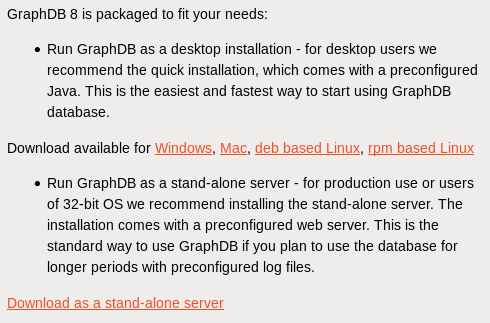
\includegraphics[width=0.4\textwidth]{img/graphdb_email.png}
        \caption{Parte do email recebido pelo GraphDB\label{fig:instalacao-email}}
    \end{figure}

    A criação da imagem \texttt{server} é necessária quando não existe ou quando o código da \acrshort{api} de dados muda.

    \item \textbf{Interface}

    Existe apenas uma imagem (\texttt{interface}) que deve ser recriada sempre que a versão da \acrshort{api} de dados (variável ambiente \texttt{API\_VERSION} do ficheiro \textit{.env} da pasta \textit{deploy}) ou o \acrshort{url} da \acrshort{api} de dados para onde a interface irá fazer os pedidos (variável ambiente \texttt{API\_URL} do ficheiro \textit{.env} da pasta \textit{deploy}) ou a versão da interface (variável ambiente \texttt{INTERFACE\_VERSION} do ficheiro \textit{.env} da pasta \textit{deploy} ou o código mude.
\end{description}

Pode associar uma \textit{tag} a cada imagem a criar, no ficheiro \textit{.env} da \acrshort{api} de dados, nas variáveis ambiente \texttt{GRAPHDB\_IMG} (imagem \texttt{graphdb}) e \texttt{SERVER\_IMG} (imagem \texttt{server}) onde deve inserir o nome do repositório do \textit{DockerHub} e a \textit{tag} a usar (\verb|<repositório>:<tag>|). Já no ficheiro \textit{.env} da interface está presente a variável ambiente \texttt{INTERFACE\_IMG} com o mesmo intuito mas para a imagem da interface. Para criar estas imagens basta correr na pasta \texttt{deploy} da \acrshort{api} de dados (para criar as imagens da \acrshort{api} de dados) ou da interface (para criar a imagem da interface):

\footnotesize
\begin{verbatim}
    docker-compose -f docker-compose-build.yml build
\end{verbatim}
\normalsize

Depois de criadas as imagens se pretender torná-las disponíveis no \textit{DockerHub} deve para cada uma delas realizar o seguinte comando:
\footnotesize
\begin{verbatim}
    docker push <repositório>:<tag>
\end{verbatim}
\normalsize

\subsubsection{Configuração}\label{sec:int-config}
Tanto na \acrshort{api} de dados como na interface na pasta \texttt{deploy} está presente um ficheiro \textit{.env} já referido. Estes ficheiros permitem configurar respetivamente a instalação da \acrshort{api} de dados e da interface.

Na \acrshort{api} de dados para além das já referidas variáveis ambiente (\texttt{GRAPHDB\_VERSION}, \texttt{GRAPHDB\_DATA\_FILE}, \texttt{GRAPHDB\_IMG} e \texttt{SERVER\_IMG}) possui também as seguintes variáveis ambiente:

\begin{table}[H]
\fontsize{10}{12}\selectfont
\begin{tabularx}{\textwidth}{|c|X|}
    \hline
    Variável Ambiente & Descrição \\ \hline
    \texttt{CERT\_FOLDER} & Pasta onde estão os ficheiros do certificado no \textit{container} \texttt{nginx} \\ \hline
    \texttt{ACME\_FOLDER} & Pasta onde estão os ficheiros do \texttt{acme.sh} no \textit{container} \texttt{nginx} \\ \hline
    \texttt{API\_VERSION} & Versão da \acrshort{api} de dados \\ \hline
    \texttt{DOMAINS} & Domínios dos quais a \acrshort{api} de dados irá estar acessível \\ \hline
    \texttt{SWAGGER\_URL} & \acrshort{url} principal a colocar na documentação \textit{OpenAPI} (\textit{Swagger}) \\ \hline
    \texttt{INTERFACE\_HOSTS} & \textit{Hosts} das interfaces da \acrshort{clav} que podem aceder a \acrshort{api} de dados \\ \hline
    \texttt{HTTP\_PORT} & Porta \acrshort{http} em que a \acrshort{api} de dados recebe os pedidos \acrshort{http} dentro da máquina de instalação \\ \hline
    \texttt{HTTPS\_PORT} & Porta \acrshort{https} em que a \acrshort{api} de dados recebe os pedidos \acrshort{https} dentro da máquina de instalação \\ \hline
\end{tabularx}
\caption{Variáveis ambiente do ficheiro \textit{.env} da \acrshort{api} de dados sem \textit{Kong}}
\end{table}

Quanto à interface para além das já referidas variáveis ambiente (\texttt{API\_VERSION}, \texttt{API\_URL}, \texttt{INTERFACE\_VERSION} e \texttt{INTERFACE\_IMG}) possui também as seguintes variáveis ambiente:

\begin{table}[H]
\fontsize{10}{12}\selectfont
\begin{tabularx}{\textwidth}{|c|X|}
    \hline
    Variável Ambiente & Descrição \\ \hline
    \texttt{CERT\_FOLDER} & Pasta onde estão os ficheiros do certificado no \textit{container} \texttt{interface} \\ \hline
    \texttt{ACME\_FOLDER} & Pasta onde estão os ficheiros do \texttt{acme.sh} no \textit{container} \texttt{interface} \\ \hline
    \texttt{DOMAINS} & Domínios dos quais a interface irá estar acessível \\ \hline
    \texttt{SERVER\_URL} & \acrshort{url} da \acrshort{api} de dados \\ \hline
    \texttt{HTTP\_PORT} & Porta \acrshort{http} em que a interface recebe os pedidos \acrshort{http} dentro da máquina de instalação \\ \hline
    \texttt{HTTPS\_PORT} & Porta \acrshort{https} em que a interface recebe os pedidos \acrshort{https} dentro da máquina de instalação \\ \hline
    \texttt{NGINX\_FILE} & Ficheiro de configuração \textit{Nginx} a usar. Duas hipóteses:
    \begin{itemize}
        \item \texttt{nginx.conf.template}: A interface não faz redirecionamento dos pedidos que recebe para a \acrshort{api} de dados. O valor de \texttt{API\_URL} tem de ser o \acrshort{url} real da \acrshort{api} de dados (será igual a \texttt{SERVER\_URL})
        \item \texttt{nginxProxy.conf.template}: A interface faz redirecionamento dos pedidos que recebe para a \acrshort{api} de dados. O valor de \texttt{API\_URL} tem de ser o \acrshort{url} da interface, estando em \texttt{SERVER\_URL} o \acrshort{url} real da \acrshort{api} de dados
    \end{itemize}
    \\ \hline
\end{tabularx}
\caption{Variáveis ambiente do ficheiro \textit{.env} da interface}
\end{table}

Tanto na \acrshort{api} de dados como na interface, caso sejam alteradas estas variáveis ambiente não é necessário recriar as imagens, basta apenas reiniciar os \textit{containers}.

Após realizar as alterações necessárias pode correr o seguinte comando na pasta \texttt{deploy} da \acrshort{api} de dados (para iniciar a \acrshort{api} de dados) ou da interface (para iniciar a interface):

\footnotesize
\begin{verbatim}
    docker-compose up
\end{verbatim}
\normalsize

Este comando também funciona mesmo que as imagens não estejam criadas desde que estejam presentes no \textit{DockerHub} (verifica de acordo com os valores das variáveis ambiente \texttt{GRAPHDB\_IMG} e \texttt{SERVER\_IMG} na \acrshort{api} e \texttt{INTERFACE\_IMG} na interface).

Caso as imagens (\texttt{server} e \texttt{graphdb} ou \texttt{interface}) ainda não estejam criadas (nem presentes no \textit{DockerHub}) pode criá-las e de seguida iniciá-las através do comando:

\footnotesize
\begin{verbatim}
    docker-compose -f docker-compose-build.yml up
\end{verbatim}
\normalsize

Na \acrshort{api} de dados se pretende manter os dados entre atualizações (criação de novas imagens e reinícios dos \textit{containers}) não deve eliminar os volumes \texttt{clav-mongodb-data} (dados da \acrshort{bd} \textit{MongoDB}) e \texttt{clav-graphdb-data} (dados da \acrshort{bd} \textit{GraphDB}). Além disso, não deve eliminar os volumes \texttt{acme-data} e \texttt{crontabs}, o primeiro para não ser necessário gerar novos certificados (podendo atingir o limite de geração de certificados do \textit{Let's Encrypt}) e o segundo visto ser o ficheiro de configuração que permite que execute periodicamente (diariamente) o \texttt{acme.sh} para verificar se os certificados tem apenas 30 dias de validade e como tal proceder à renovação destes.

Do lado da interface os volumes que não deve eliminar são \texttt{acme-interface-data} e \texttt{crontabs-interface} pelas mesmas razões já referidas para os volumes \texttt{acme-data} e \texttt{crontabs}. 

\subsubsection{Povoamento do \textit{MongoDB}}\label{sec:inst-povMDB}
Até ao momento nesta instalação a \acrshort{bd} \textit{MongoDB} continua vazia. Se já possui uma \acrshort{bd} do \textit{MongoDB} já povoada é possível proceder à migração. Caso contrário precisará de pelo menos inserir à mão (através do cliente do \textit{MongoDB}) um utilizador com o nível de Administrador de Perfil Tecnológico à coleção \texttt{users} caso contrário será impossível registar/inserir utilizadores pela interface já que apenas pessoal registado e com determinado nívelpode registar/inserir utilizadores.

\begin{description}
    \item \textbf{Backup}

    De forma a realizar a migração é necessário primeiro fazer o backup da \acrshort{bd} já povoada. Para realizar o backup executa-se o comando seguinte:
    \footnotesize
    \begin{verbatim}
    mongodump --db <nome da BD> --out <caminho a guardar o backup>
    \end{verbatim}
    \normalsize
    \vspace{-0.5cm}
    No destino final será criada uma pasta com o nome da \acrshort{bd} que irá possuir o backup da \acrshort{bd}.
    Para se poder realizar backup é necessário que o \textit{MongoDB} esteja a correr.
    \item \textbf{Importação da informação}

    Primeiro, é necessário parar \textit{containers}:
    \footnotesize
    \begin{verbatim}
    docker stop clav_nginx
    docker stop clav_server
    docker stop clav_mongo clav_graphdb
    \end{verbatim}
    \normalsize
    \vspace{-0.3cm}
    Para importar os dados nesta instalação basta executar o seguinte comando:
    \footnotesize
    \begin{verbatim}
    docker run --rm -v clav-mongodb-data:/data/db \
        -v <caminho absoluto onde foi guardado o backup>/<nome da BD>:/backup mongo \
        bash -c "(mongod &) && mongorestore --db <nome da BD> --drop /backup"
    \end{verbatim}
    \normalsize
    \vspace{-0.3cm}
    No fim, é necessário voltar a iniciar os \textit{containers}:
    \footnotesize
    \begin{verbatim}
    docker start clav_mongo clav_graphdb
    docker start clav_server
    docker start clav_nginx
    \end{verbatim}
    \normalsize
    \vspace{-0.5cm}
\end{description}

\subsubsection{Melhorias de segurança do \acrshort{https}}\label{sec:inst-melhorias}
Após concluir a instalação recomenda-se duas melhorias de segurança do \acrshort{https} onde uma delas apenas se pode realizar agora. Nesta secção quando se refere o domínio ou domínios pretende-se fazer referência aos presentes nos \texttt{DOMAINS} dos ficheiros de configuração \textit{.env} da \acrshort{api} de dados e da interface.

A melhoria apenas agora possível é a adição dos domínios à \textit{\acrshort{hsts} preload list}. Para isso deve aceder a \url{https://hstspreload.org/}, começar por inserir um dos domínios e seguir os passos indicados. Repita para os restantes domínios. O \textit{\acrshort{hsts} preloading} permite que os \textit{browsers} saibam à partida que dominíos devem ser acedidos apenas por \acrshort{https}.\footnote{Ver \url{https://scotthelme.co.uk/hsts-preloading/} para perceber esta melhoria de segurança} 

A outra melhoria de segurança é a adição de \textit{\acrshort{caa} records} associados aos domínios no \acrshort{dns} (tem de suportar \textit{\acrshort{caa} records}) no qual os domínios estão indexados. Os \textit{\acrshort{caa} records} a adicionar podem ser obtidos em \url{https://sslmate.com/caa/} indicando o nome do domínio e escolhendo como \textit{Authorized Certificate Authorities} o \textit{Let's Encrypt}. Na secção 4 da página Web estará presente os \textit{\acrshort{caa} records} a adicionar. Repita para os restantes domínios. Estes \textit{\acrshort{caa} records} indicam a(s) autoridade(s) emissora(s) de certificados permitida(s) para o(s) domínio(s) por forma a impedir a emissão de um certificado para o(s) mesmo(s) domínio(s) noutra autoridade emissora de certificados.\footnote{Ver \url{https://sslmate.com/caa/about} para perceber esta melhoria de segurança} 

\subsection{Atualizações}\label{sec:inst-update}

Tal como a instalação, as atualizações podem ser feitas de forma separada, ou seja, é possível atualizar apenas a \acrshort{api} de dados ou apenas a interface ou até as duas se assim o pretender.

Para tal, deve-se primeiro parar os \textit{containers}:

\footnotesize
\begin{center}
\begin{minipage}[t]{0.4\textwidth}
\acrshort{api} de dados:
\begin{verbatim}
docker stop clav_nginx
docker stop clav_server
docker stop clav_mongo clav_graphdb
\end{verbatim}
\end{minipage}%
\begin{minipage}[t]{0.4\textwidth}
Interface:
\begin{verbatim}
docker stop interface
\end{verbatim}
\end{minipage}
\end{center}
\normalsize

Antes de recriar as imagens se pretender colocá-las no \textit{DockerHub} deve alterar as \textit{tags} nos ficheiros de configuração \textit{.env} da(s) imagem(s) que precisará de recriar por forma a não sobescrever \textit{tags}. Fica à escolha do utilizador. Apenas tem de ter em conta que as variáveis ambiente \texttt{GRAPHDB\_IMG}, \texttt{SERVER\_IMG} e \texttt{INTERFACE\_IMG} podem ser utilizadas para gerir as imagens da forma que pretender.

De seguida recria-se os \textit{containers} necessários:
\begin{itemize}
    \item Caso tenha mudado a ontologia ou pretenda atualizar a distribuição do \textit{GraphDB} recria-se a imagem do \texttt{clav\_graphdb} após as devidas alterações no ficheiro \textit{.env} da pasta \textit{deploy}:
    \footnotesize
    \begin{verbatim}
    docker-compose -f docker-compose-build.yml build graphdb
    \end{verbatim}
    \normalsize
    \vspace{-0.4cm}
    No caso do ficheiro da ontologia ter sido alterado é necessário correr também:
    \footnotesize
    \begin{verbatim}
    docker rm clav_graphdb
    docker volume rm clav-graphdb-data
    \end{verbatim}
    \normalsize
    \vspace{-0.5cm}
    \item Caso tenha sido alterado código na \acrshort{api} de dados (\verb|git pull|) recria-se a imagem do \texttt{clav\_server}:
    \footnotesize
    \begin{verbatim}
    git pull #obter novos commits
    docker-compose -f docker-compose-build.yml build server
    \end{verbatim}
    \normalsize
    \vspace{-0.5cm}
    \item Caso tenha sido alterado código da interface (\verb|git pull|) ou uma das variáveis ambientes \texttt{API\_URL} e/ou \texttt{API\_VERSION} tenham sido alteradas recria-se a imagem da \texttt{interface}:
    \footnotesize
    \begin{verbatim}
    git pull #obter novos commits
    docker-compose -f docker-compose-build.yml build interface
    \end{verbatim}
    \normalsize
    \vspace{-0.5cm}
\end{itemize}
Caso o \textit{build} use a \textit{cache} para construir as imagens adicione a \textit{flag} \verb|--no-cache| no comando de \textit{build} (a seguir à palavra \textit{build}).

Por fim, inicia-se os \textit{containers} da \acrshort{api} de dados ou da interface dependendo em que pasta \texttt{deploy} está através do comando:
\footnotesize
\begin{verbatim}
    docker-compose up -d
\end{verbatim}
\normalsize

Note que, a opção \texttt{-d} é necessária para o comando libertar novamente a consola e colocar os \textit{containers} a correr em background.

\subsection{Backup}\label{sec:inst-backup}

Em termos de backup, os volumes de maior importância são o do \textit{MongoDB} e o do \textit{GraphDB} visto possuírem toda a informação da \acrshort{clav}. Note que este backup apenas implica a \acrshort{api} de dados. Por forma a realizar o backup deve:
\begin{lstlisting}[caption=Backup dos volumes do \textit{docker}]
    #parar containers
    docker stop clav_nginx
    docker stop clav_server
    docker stop clav_mongo clav_graphdb
    
    #backup do volume do GraphDB
    docker run --rm --volumes-from clav_graphdb \
        -v $(pwd):/backup ubuntu \
        bash -c "cd /opt/graphdb/home/data/repositories && \
        tar cvf /backup/clav_graphdb.tar ."
        
    #backup do volume do MongoDB
    docker run --rm --volumes-from clav_mongo \
        -v $(pwd):/backup ubuntu bash -c "cd /data/db && \
        tar cvf /backup/clav_mongo.tar ."
        
    #Pode agora iniciar os containers
    docker start clav_mongo clav_graphdb
    docker start clav_server
    docker start clav_nginx
\end{lstlisting}

No final possuirá dois ficheiros \acrshort{tar} (\texttt{clav\_graphdb.tar} e \texttt{clav\_mongo.tar}) na raiz onde executou os comandos que são respetivamente o backup do \textit{GraphDB} e o backup do \textit{MongoDB}.

A partir daqui pode armazenar estes onde achar mais conveniente e seguro.

\subsection{Migração}\label{sec:inst-migracao}

Para realizar a migração para outra máquina é necessário primeiro realizar o backup dos volumes da máquina atual. Pode para isso seguir a descrição dada na secção~\ref{sec:inst-backup}. Depois deve copiar os ficheiros comprimidos (\acrshort{tar}) para a nova máquina de instalação.

Os passos seguintes serão a realização da primeira instalação na nova máquina, bastando para isso seguir descrição dada na secção~\ref{sec:inst-prim} mas sem realizar o povoamento do \textit{MongoDB}.

O passo final é restaurar os volumes através dos backups (ficheiros comprimidos). Para tal siga os seguintes passos para restaurar os volumes:
\begin{lstlisting}[caption=Restauro dos volumes do \textit{docker}]
    #assumindo que se encontra na raiz onde se encontram os ficheiros TAR

    #parar containers
    docker stop clav_nginx
    docker stop clav_server
    docker stop clav_mongo clav_graphdb
    
    #restauro do volume do GraphDB
    docker run --rm -v clav-graphdb-data:/opt/graphdb/home/data/repositories \
        -v $(pwd):/backup ubuntu bash -c "cd /opt/graphdb/home/data/repositories \
        && tar xvf /backup/clav_graphdb.tar"
        
    #restauro do volume do MongoDB
    docker run --rm -v clav-mongodb-data:/data/db \
        -v $(pwd):/backup ubuntu bash -c "cd /data/db \
        && tar xvf /backup/clav_mongo.tar"
        
    #voltar a iniciar os containers
    docker start clav_mongo clav_graphdb
    docker start clav_server
    docker start clav_nginx
\end{lstlisting}

Pode também dividir a \acrshort{api} de dados e a interface por duas máquinas. Para isso deve realizar na mesma o backup dos volumes na máquina atual, seguir a primeira instalação individualmente para cada máquina (instalando apenas a componente correspondente), copiar os backups apenas para a máquina da \acrshort{api} de dados e restaurar esses backups.

\section{Versão com \textit{Kong}}\label{sec:deployKong}

Nesta versão será apenas abordado a instalação da \acrshort{api} de dados já que a adição do \textit{Kong} não implicou qualquer alteração na interface.

\subsection{Primeira instalação}

Os dois primeiros passos são exatamente iguais aos já descritos na primeira instalação da versão sem \textit{Kong} (ver~\ref{sec:inst-prim}), instalar as dependências necessárias e abrir as portas na máquina de instalação para a \acrshort{api} de dados.

De seguida realiza-se a clonagem do repositório \texttt{git}, muda-se de raiz e de \textit{branch}:

\footnotesize
\begin{verbatim}
    git clone https://github.com/jcm300/docker-clav.git
    cd docker-clav
    git checkout kong
\end{verbatim}
\normalsize

Além disso, obtém-se o conteúdo dos submódulos do repositório ao correr:

\footnotesize
\begin{verbatim}
    git submodule update --init
\end{verbatim}
\normalsize

Tal como na versão sem \textit{Kong}, numa versão de produção é necessário gerar dois novos pares de chaves pública/privada e copiar as novas chaves públicas para interface:

\footnotesize
\begin{center}
\begin{minipage}[t]{0.49\textwidth}
Gerar dois pares de chaves pública/privada:
\begin{verbatim}
#assume-se que se encontra na pasta docker-clav 
openssl genrsa -out CLAV-auth/config/keys/apiKey 2048
openssl rsa -in CLAV-auth/config/keys/apiKey -pubout \
    -out CLAV-auth/config/keys/apiKey.pub
openssl genrsa -out CLAV-auth/config/keys/userKey 2048
openssl rsa -in CLAV-auth/config/keys/userKey -pubout \
    -out CLAV-auth/config/keys/userKey.pub
\end{verbatim}
\end{minipage}%
\begin{minipage}[t]{0.49\textwidth}
Na interface copiar para esta as chaves públicas geradas (este comando apenas funciona se a \acrshort{api} e a interface estão na mesma máquina):
\begin{verbatim}
#assume-se que se encontra na pasta docker-clav 
cp CLAV-auth/config/keys/apiKey.pub \
    CLAV-auth/config/keys/userKey.pub \
    <raíz da pasta da interface>/src/plugins/keys/
\end{verbatim}
\end{minipage}
\end{center}
\normalsize

\subsubsection{Criação de Imagens}

A criação da imagem \texttt{graphdb} não sofre muitas alterações em relação à versão sem \textit{Kong} (ver~\ref{sec:int-imagens}). Algumas das diferenças a ter em conta são que a pasta \texttt{graphdb} e o ficheiro \textit{.env} encontram-se na pasta \texttt{docker-clav}. A criação da imagem \texttt{server} não sofreu quaisquer alterações.

A maior diferença desta versão em relação à versão sem \textit{Kong} é a necessidade de também criar a imagem \texttt{clav-auth} que, como a imagem \texttt{server}, apenas necessita de ser criada quando não existe ou quando o seu código muda.

\subsubsection{Configuração}

No ficheiro \textit{.env} desta versão para além das variáveis ambiente \texttt{GRAPHDB\_VERSION}, \texttt{GRAPHDB\_DATA\_FILE}, \texttt{GRAPHDB\_IMG} e \texttt{SERVER\_IMG} com o mesmo intuito da versão sem \textit{Kong} há as seguintes variáveis ambiente:

\begin{table}[H]
\fontsize{10}{12}\selectfont
\begin{tabularx}{\textwidth}{|c|X|}
    \hline
    Variável Ambiente & Descrição \\ \hline
    \texttt{SERVER\_AUTH\_IMG} & Tem a mesma finalidade que a variável \textit{SERVER\_IMG} mas para o servidor de autenticação \\ \hline
    \texttt{EMAIL} & Email a usar para gerar os certificados \\ \hline
    \texttt{API\_VERSION} & Versão da \acrshort{api} de dados \\ \hline
    \texttt{DOMAINS} & Domínios dos quais a \acrshort{api} de dados irá estar acessível \\ \hline
    \texttt{INTERFACE\_HOSTS} & \textit{Hosts} das interfaces da \acrshort{clav} que podem aceder \\ \hline
    \texttt{HTTP\_PORT} & Porta \acrshort{http} em que a \acrshort{api} de dados recebe os pedidos \acrshort{http} dentro da máquina de instalação \\ \hline
    \texttt{HTTPS\_PORT} & Porta \acrshort{https} em que a \acrshort{api} de dados recebe os pedidos \acrshort{https} dentro da máquina de instalação \\ \hline
\end{tabularx}
\caption{Variáveis ambiente do ficheiro \textit{.env} da \acrshort{api} de dados com \textit{Kong}}
\end{table}

Caso sejam alteradas estas variáveis ambiente (tirando \texttt{SERVER\_AUTH\_IMG}) não é necessário recriar as imagens, basta apenas reiniciar os \textit{containers}.

Após realizar as alterações necessárias, para criar as imagens e iniciar a \acrshort{api} de dados basta correr:

\footnotesize
\begin{verbatim}
    docker-compose -f docker-compose-build.yml up
\end{verbatim}
\normalsize

Caso as imagens já estejam criadas ou estejam presentes no \textit{DockerHub} pode correr:

\footnotesize
\begin{verbatim}
    docker-compose up
\end{verbatim}
\normalsize

De igual forma como na versão sem \textit{Kong} não deve eliminar os volumes \texttt{clav-mongodb-data} (dados da \acrshort{bd} \textit{MongoDB}), \texttt{clav-graphdb-data} (dados da \acrshort{bd} \textit{GraphDB}) e, além dessas, não deve eliminar \texttt{clav-acme-data} (dados referentes aos certificados e à configuração destes).

\subsubsection{Povoamento do \textit{MongoDB}}

O povoamento do \textit{MongoDB} pode ser efetuado de igual forma como na primeira instalação sem \textit{Kong} (ver~\ref{sec:inst-povMDB}). As únicas diferenças é que para parar os \textit{containers} deve executar:

\footnotesize
\begin{verbatim}
    docker stop clav_kong
    docker stop clav_redis clav_auth clav_server
    docker stop clav_mongo clav_graphdb
    \end{verbatim}
\normalsize
\vspace{-0.5cm}

e para iniciar os \textit{containers} deve correr:

\footnotesize
    \begin{verbatim}
    docker start clav_mongo clav_graphdb
    docker start clav_redis clav_auth clav_server
    docker start clav_kong
    \end{verbatim}
\normalsize
\vspace{-0.5cm}

\subsubsection{Melhorias de segurança do \acrshort{https}}

Quanto às melhorias de segurança são iguais e são aplicadas de igual forma como na versão sem \textit{Kong} (ver~\ref{sec:inst-melhorias}).

\subsection{Atualizações}

Numa atualização com \textit{Kong} um dos primeiros passos é verificar se há atualizações:
\footnotesize
\begin{verbatim}
    #assumindo que se encontra na pasta docker-clav
    git pull #obter novos commits
\end{verbatim}
\normalsize

De resto as únicas diferenças em relação à versão sem \textit{Kong} (ver~\ref{sec:inst-update}) são o código a executar para parar os \textit{containers}. Além disso, tal como a imagem do \texttt{clav\_server}, quando o código do serviço de autenticação muda é necessário recriar a imagem do \texttt{clav-auth}:

\footnotesize
\begin{verbatim}
    #assumindo que se encontra na pasta docker-clav
    cd CLAV-auth
    git pull origin master #obter novos commits
    cd ..
    docker-compose -f docker-compose-build.yml build clav-auth
\end{verbatim}
\normalsize

Por fim, outra diferença é que para recriar a imagem do \texttt{clav\_server} deve executar:

\footnotesize
\begin{verbatim}
    #assumindo que se encontra na pasta docker-clav
    cd CLAV2018
    git pull origin kong #obter novos commits
    cd ..
    docker-compose -f docker-compose-build.yml build server
\end{verbatim}
\normalsize

\subsection{Backup}

No backup as únicas diferenças em relação à versão sem \textit{Kong} (ver~\ref{sec:inst-backup}) são o código a executar para parar e para iniciar os \textit{containers}.

\subsection{Migração}

Na migração será seguir a primeira instalação desta versão. De resto, os passos serão iguais aos apresentados na versão sem \textit{Kong} (ver~\ref{sec:inst-migracao}) tirando o código para parar e para iniciar os \textit{containers}.

\section{Versão sem \textit{Kong} vs com \textit{Kong}}

Esta secção tem como objetivo realizar uma comparação entre as duas versões com o objetivo de decidir qual delas se adequa mais.

Para realizar os testes nesta secção, cada componente foi executado numa máquina do \textit{Digital Ocean} com \textit{Ubuntu 20.04 x64}, 8 GB de memória \acrshort{ram} e 4 \acrshort{cpu}s. Para traduzir o domínio no \acrshort{ip} da máquina foi usado o \textit{No-IP}\footnote{ver \url{https://www.noip.com/}}.

Para comparar a performance foi realizado um teste em que 100 utilizadores fazem dois pedidos, um pedido das classes e quando termina um pedido de uma classe específica. Um utilizador começa os seus pedidos 1 segundo após o anterior. Para realizar este teste foi usado o \textit{Apache JMeter}. Os resultados obtidos foram os seguintes (atenção que a \textit{cache} estava ``quente'' nas duas versões, portanto o pedido das classes deverá ser proveniente da cache):

\begin{table}[H]
    \footnotesize
    \centering
    \begin{tabular}{| c | c | c | c | c | }
        \hline
        Versão \acrshort{api} & Pedido & Tempo de Resposta (média em ms) & \% de Erro & \textit{Throughput} (pedidos por) \\ \hline
        \multirow{3}{*}{sem \textit{Kong}} & Classes & 1650 & 0 & 59.9/min \\ \cline{2-5}
        & Classe & 465 & 0 & 1.0/s \\ \cline{2-5}
        & Total & 1057 & 0 & 2.0/s \\ \hline
        \multirow{3}{*}{com \textit{Kong}} & Classes & 2469 & 0 & 59.6/min \\ \cline{2-5}
        & Classe & 588 & 0 & 1.0/s \\ \cline{2-5}
        & Total & 1529 & 0 & 2.0/s \\ \hline
    \end{tabular}
    \caption{Resultados de performance para a \acrshort{api} de dados}
\end{table}

Olhando para os resultados, o \textit{throughput} é bastante semelhante entre as duas, contudo o tempo de resposta é menor na versão sem \textit{Kong}, o que faz algum sentido já que a versão com \textit{Kong} (o \textit{Kong} tem embutido o \textit{Nginx}) é mais pesada em termos de componentes em execução.

Em termos de facilidade de instalação, as duas são bastante semelhantes pelo que quem conseguir instalar com uma delas consegue instalar a outra.

Quanto à proteção da \acrshort{api} apesar das várias alterações (componente externo à \acrshort{api} de dados), são semelhantes tendo como principal diferença o não uso do \texttt{passport} na versão com \textit{Kong} o que não afeta a forma como é realizada a proteção. De certa forma, o uso do \texttt{passport} na versão sem \textit{Kong} é atualmente desnecessária desde que se coloque em \texttt{req.user} a informação presente no \textit{token} do utilizador. A essência da proteção da \acrshort{api} de dados manteve-se basicamente igual.

\subsection{Configuração do \acrshort{https}}

A plataforma \textit{SSL Labs} possui uma ferramenta \textit{online} que permite-nos auferir a qualidade da configuração do \acrshort{https} num domínio.\footnote{Ver \url{https://www.ssllabs.com/ssltest/}} Para perceber melhor a classificação realizada pelo \textit{SSL Labs} recomenda-se a leitura de \url{https://github.com/ssllabs/research/wiki/SSL-Server-Rating-Guide}.

Nesta secção foi também comparada a configuração do \acrshort{https} da interface para além das versões da \acrshort{api}:
\begin{figure}[H]
    \centering
    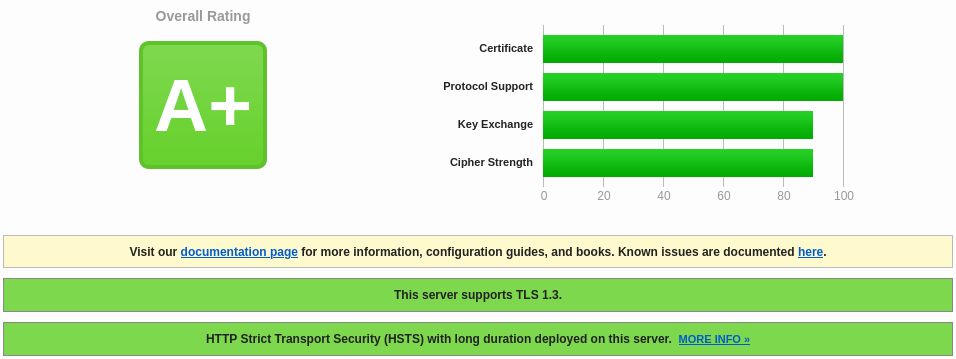
\includegraphics[width=0.6\textwidth]{img/sslLabsAPISemKong.png}
    \caption{Classificação \textit{SSL Labs} da \acrshort{api} sem \textit{Kong}}
\end{figure}
\begin{figure}[H]
    \centering
    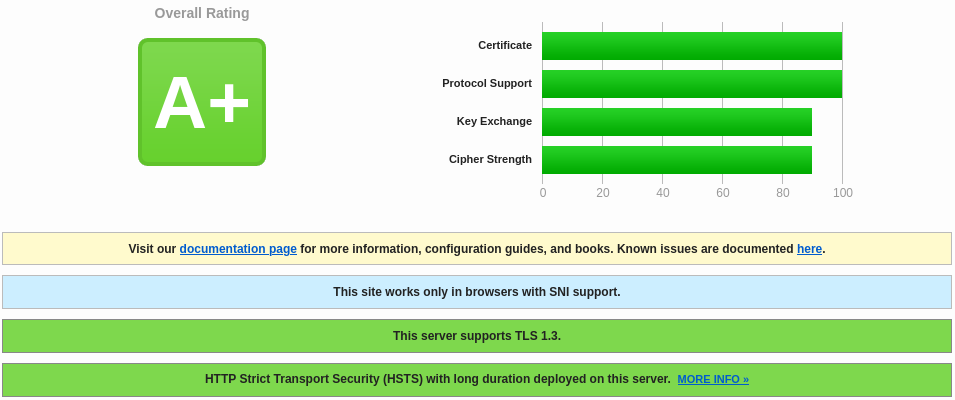
\includegraphics[width=0.6\textwidth]{img/sslLabsAPIComKong.png}
    \caption{Classificação \textit{SSL Labs} da \acrshort{api} com \textit{Kong}}
\end{figure}
\begin{figure}[H]
    \centering
    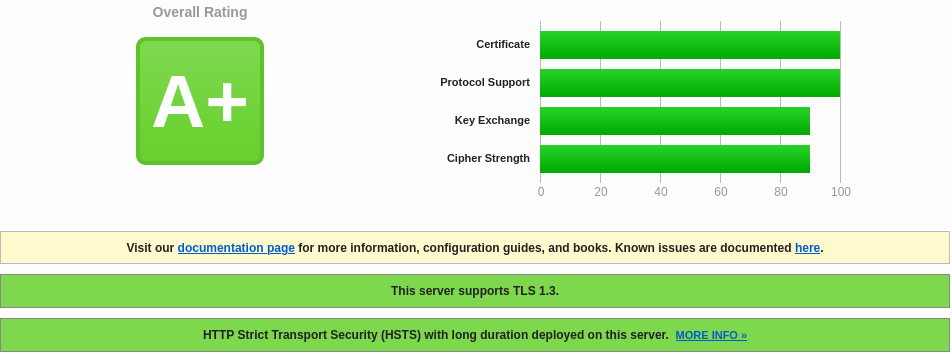
\includegraphics[width=0.6\textwidth]{img/sslLabsInterface.png}
    \caption{Classificação \textit{SSL Labs} da Interface}
\end{figure}

Como é possível verificar pelas imagens as 3 tem a classificação máxima, A+, bem como a mesma classificação em cada componente específica. A \acrshort{api} sem \textit{Kong} é normal ter a mesma classificação que a interface porque a configuração usada é praticamente a mesma. Quanto ao caso da \acrshort{api} de dados com \textit{Kong} esta apenas funciona em \textit{browsers} que suportam \acrshort{sni} o que são raros já que quase todos suportam atualmente. Além disso a versão com \textit{Kong} não tem ativado o \acrshort{ocsp} \textit{stapling} (uma das recomendações de segurança) enquanto que nos outros casos esta está ativa. Estas duas diferenças da versão com \textit{Kong} devem-se à forma como o \textit{Kong} e o \textit{plugin} do \textit{Kong} \texttt{acme} funcionam.

Por fim, nos 3 casos há um único sinal de aviso, que se deve à falta do \textit{\acrshort{caa} record} (uma das melhorias de segurança referidas) no \acrshort{dns}. Contudo, com os resultados obtidos conseguimos ter alguma certeza de que as configurações realizadas são atualmente seguras.

\subsection{Resumo}

Em conclusão, apesar de a configuração do \acrshort{https} da \acrshort{api} com \textit{Kong} ser ligeiramente pior bem como a performance (tempo de resposta), em termos gerais permite obter futuramente uma melhor \acrshort{api}, com uma maior modularidade. Permite também futuramente escalar mais facilmente a \acrshort{api} de dados bem como modularizar esta \acrshort{api} em mais componentes.

\section{Resumo}

Neste capítulo foi descrito o procedimento de instalação da \acrshort{api} sem \textit{Kong}, da \acrshort{api} com \textit{Kong} e da interface. No fim é feita uma comparação entre as duas versões da \acrshort{api}, concluindo que no nosso caso se adequa mais a versão com \textit{Kong}.
